%%%%%%%%%%%%%%%%%%%%%%%%%%%%%%%%%%%%%%%%%%%%%%%%%%
%% Authors :    Giovanni Arcari                 %%
%%              Mariia Bronzova                  %%
%%              Luca Sardi                      %%
%%              Spencer Sharp                   %%
%%                                              %%
%% Supervisor : Andreas Apostolatos             %%
%%											  	%%
%% e-mail : andreas.apostolatos@tum.de		   	%%
%%											  	%%
%% 09_Appendix.tex					  	   	  	%%
%%											  	%%
%%%%%%%%%%%%%%%%%%%%%%%%%%%%%%%%%%%%%%%%%%%%%%%%%%
\section{APPENDIX}

Included in the Appendix are two sections. First, the implemented Matlab code is illustrated graphically through a series of flowcharts. Second, the basic process of using GiD is broken down, and the enhancements that were implemented are discussed.
%%%%%%%%%%%%%%%%%%%%%%%%%%%%%% MATLAB %%%%%%%%%%%%%%%%%%%%%%%%%%%%%%%%
\subsection{Matlab Code} \label{section:appendix_matlab}
In this section different flowcharts will be presented. These flowcharts make no claim to completeness as certain things (i.e. initiation of matrices and vectors) are partly skipped while others simplified but is instead intended to give an overview of some aspects of the code at hand. Together with the code itself which was commented thoroughly the understanding of the reader should be eased.\\[3pt]
The first flowchart, Figure \ref{fig:Main}, provides an overview of the entire code from start to finish. It demonstrates how the user selection in GiD determines whether or not the sensitivity analysis and/or optimization scripts are run.\\[3pt]
\begin{figure}[ht]
  \centering
  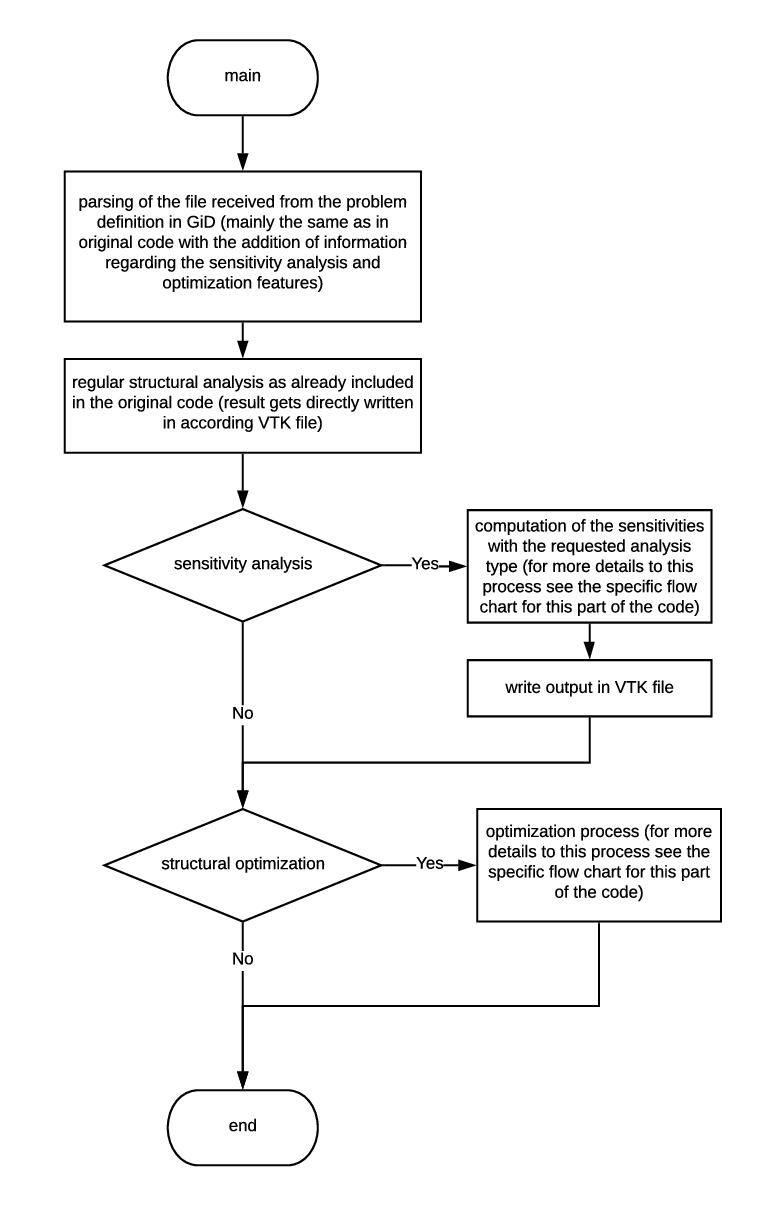
\includegraphics[width=90mm]{images/main.png}
  \caption{overview of the entire code structure}
  \label{fig:Main}
\end{figure}
The second flowchart, Figure \ref{fig:MainSensitivity}, delves more deeply into the sensitivity analysis that was implemented. Since the user has the opportunity to select either global, numerical adjoint, or analytical adjoint, along with forward, backward, or central differencing, the program must accommodate these combinations of selections.\\[3pt]
\begin{figure}[ht]
  \centering
  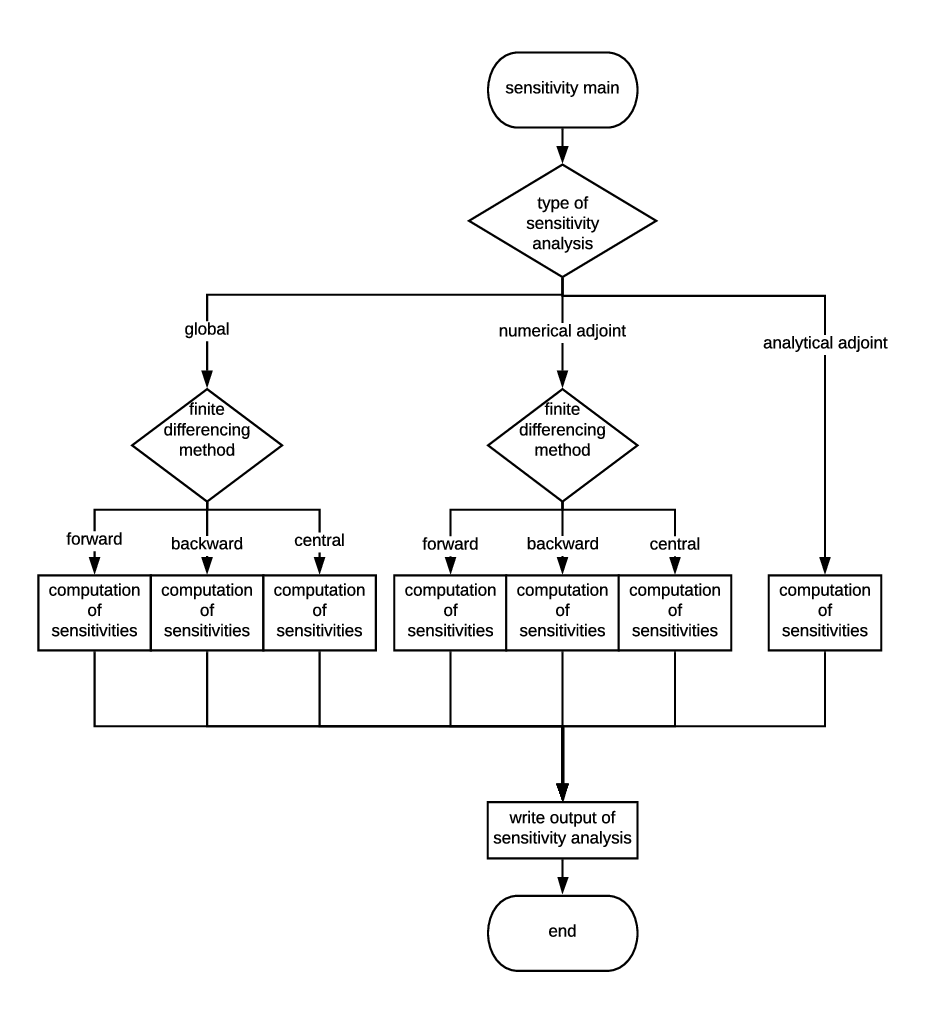
\includegraphics[width=100mm]{images/sensitivitymain.png}
  \caption{overview of the sensitivity analysis}
  \label{fig:MainSensitivity}
\end{figure}
The next flowchart, Figure \ref{fig:Global}, provides an overview of the global sensitivity analysis. As explained previously, the global sensitivity analysis requires solving the entire system $n$ times, where $n$ corresponds to the number of nodes in the structure. This process is applied for both forward and backward finite differencing.\\[3pt]
\begin{figure}[ht]
  \centering
  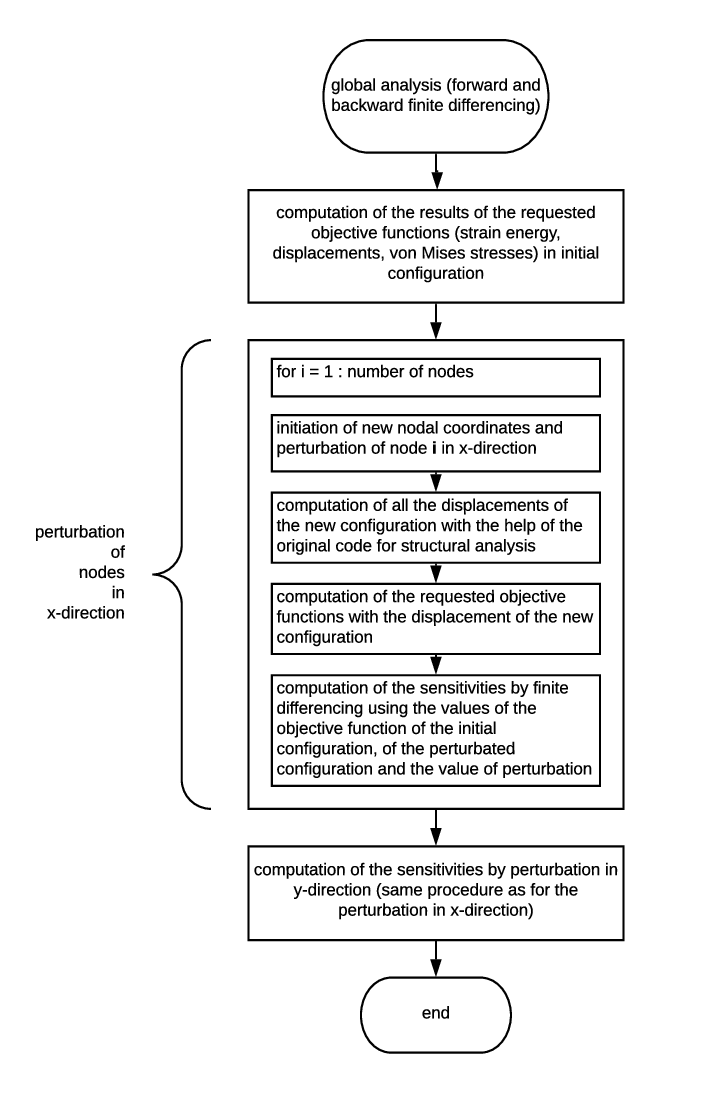
\includegraphics[width=90mm]{images/globalanalysis.png}
  \caption{global sensitivity analysis process}
  \label{fig:Global}
\end{figure}
Figure \ref{fig:Numerical} shows the process associated with the numerical adjoint sensitivity analysis. Note that whenever a derivative is computed, finite differencing is used. This process is associated with forward and backward finite differencing.\\[3pt]
Next, Figure \ref{fig:Analytical} shows the process associated with the true analytical adjoint sensitivity analysis. In contrast to the numerical adjoint method, the analytical analysis computes analytical derivatives instead of utilizing finite differencing.\\[3pt]
\begin{figure}[ht]
\centering
\begin{minipage}{.5\textwidth}
  \centering
  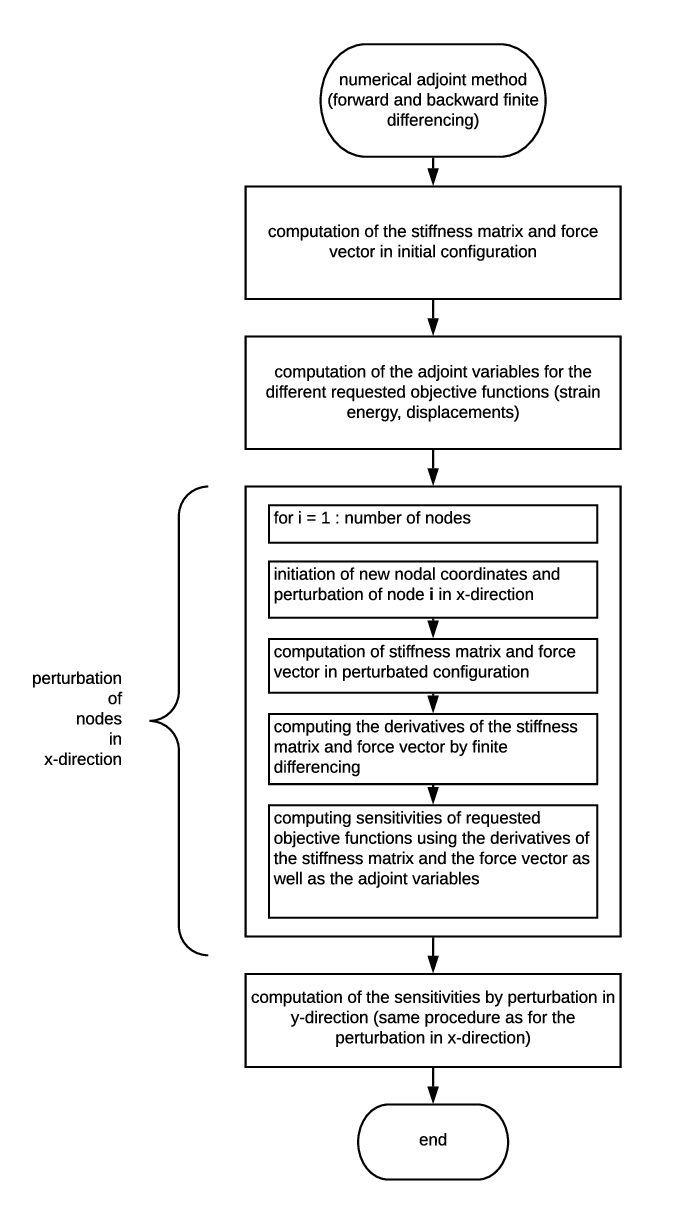
\includegraphics[width=1.0\linewidth]{images/numericaladjoint.png}
  \captionof{figure}{numerical adjoint sensitivity analysis}
  \label{fig:Numerical}
\end{minipage}%
\begin{minipage}{.5\textwidth}
  \centering
  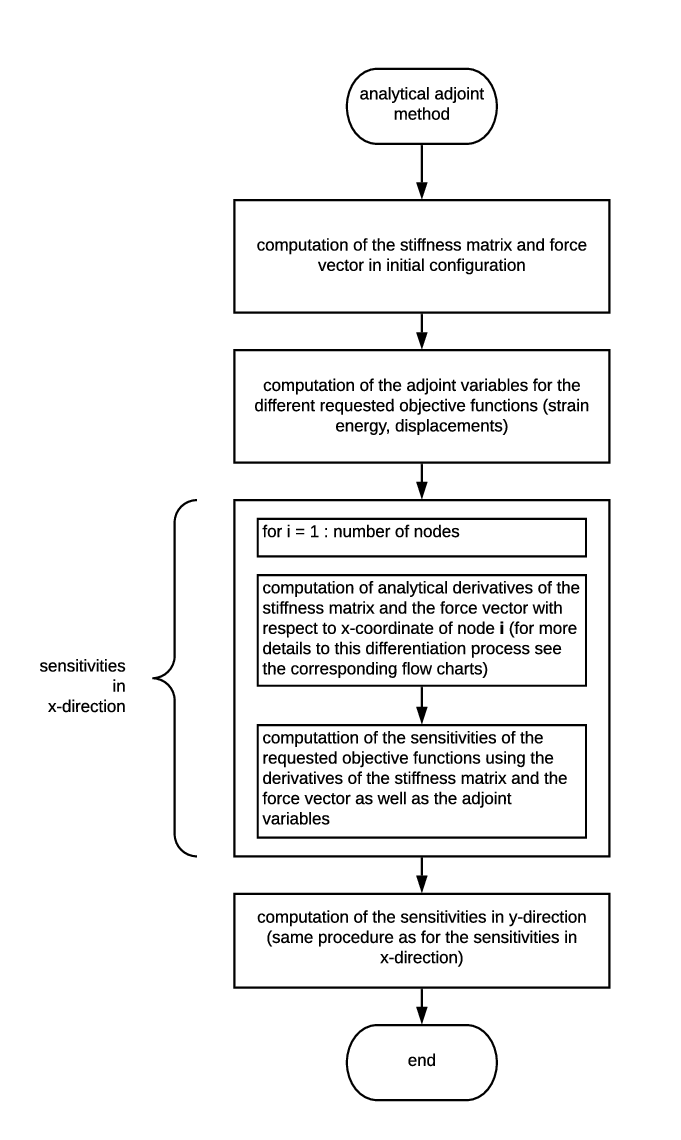
\includegraphics[width=1.07\linewidth]{images/analyticaladjoint.png}
  \captionof{figure}{analytical adjoint sensitivity analysis}
  \label{fig:Analytical}
\end{minipage}
\end{figure}
The next flowchart, Figure \ref{fig:Matrix}, outlines the process associated with the analytical differentiation of the stiffness matrix.\\[3pt]
Similarly, Figure \ref{fig:Vector} outlines the process associated with the analytical differentiation of the force vector.\\[3pt]
\begin{figure}[ht]
\centering
\begin{minipage}{.5\textwidth}
  \centering
  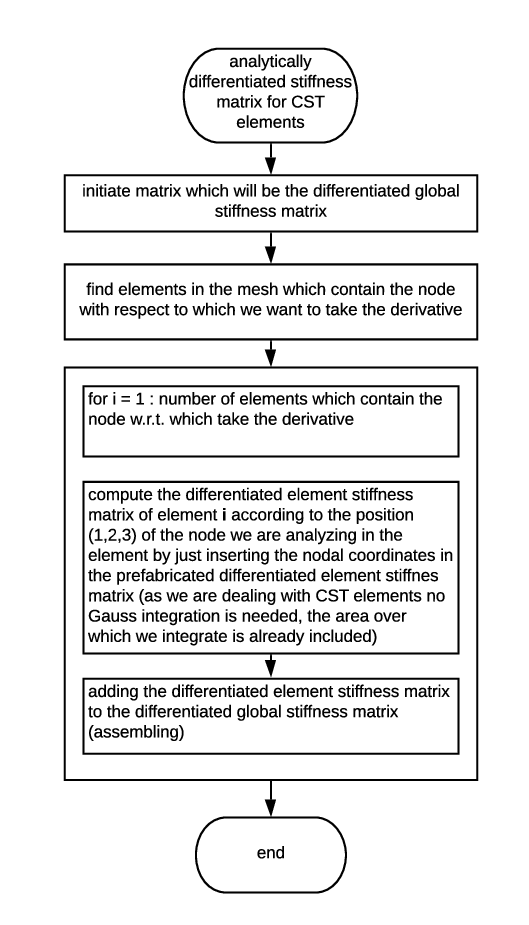
\includegraphics[width=1.06\linewidth]{images/matrixdifferentiation.png}
  \captionof{figure}{analytical stiffness matrix differentiation}
  \label{fig:Matrix}
\end{minipage}%
\begin{minipage}{.5\textwidth}
  \centering
  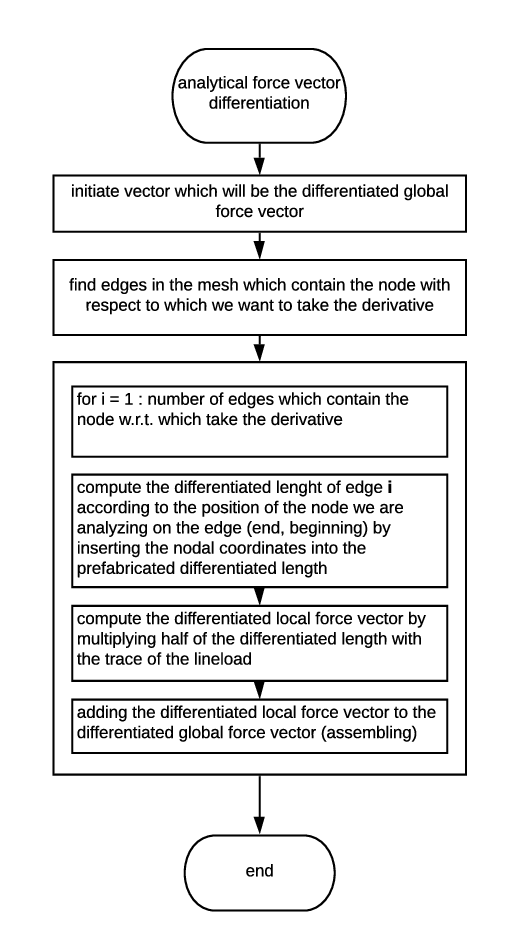
\includegraphics[width=1.0\linewidth]{images/vectordifferentiation.png}
  \captionof{figure}{analytical force vector differentiation}
  \label{fig:Vector}
\end{minipage}
\end{figure}
Finally, Figure \ref{fig:Optimization} provides an overview of the structure of the optimization code that was implemented. As described previously in section \ref{section:optimization}, the sensitivity analysis that was written can be used for the purpose of optimizing the given structure. As outlined in the flowchart, the sensitivity analysis forms the basis of the optimization algorithm as it quantifies how much each nodal coordinate should be modified.\\[3pt]
\begin{figure}[ht]
  \centering
  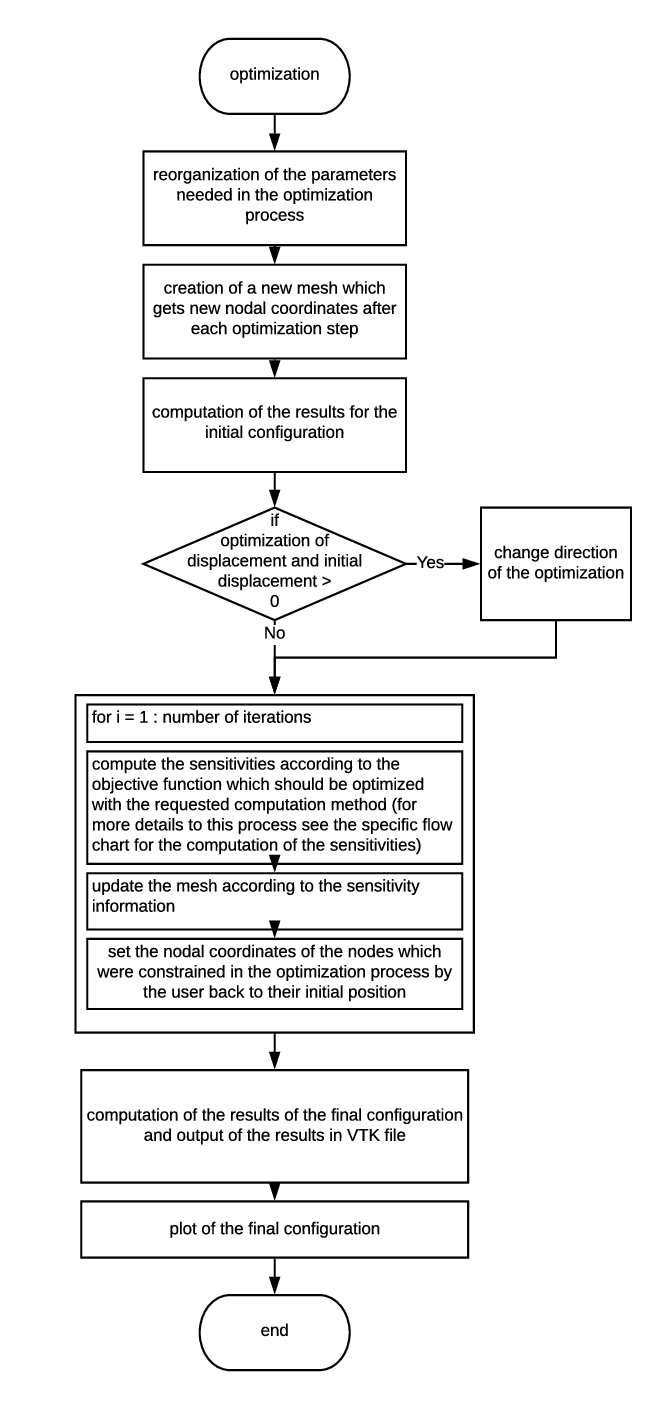
\includegraphics[width=90mm]{images/optimization.png}
  \caption{overview of the optimization code structure}
  \label{fig:Optimization}
\end{figure}
\clearpage
%%%%%%%%%%%%%%%%%%%%%%%%%%%%%%% GiD %%%%%%%%%%%%%%%%%%%%%%%%%%%%%%%%%%
\subsection{GiD GUI} \label{section:appendix_GiD}
The GiD user interface was modified as part of this assignment in order to facilitate the simple transfer of data from GiD to Matlab. The following sections provide step-by-step instructions for setting up an example problem in GiD. In order to provide a comprehensive overview, the following steps address both the original and the added functionality in the GiD user interface.

%%%%%%%%%%%%%%%%%%%%%%%%%%%% GiD - Setup %%%%%%%%%%%%%%%%%%%%%%%%%%%%%
\subsubsection{Setup}
GiD is equipped with various \texttt{problem types}, which contain the commands to customize the user interface. All of the enhancements made to GiD are within the \texttt{Matlab} problem type. When setting up a random problem, please select this as a first step, under the \texttt{Data} heading, click \texttt{Problem type} $\rightarrow$ \texttt{matlab}. See Figure \ref{fig:Matlabproblemtype}.\\
\begin{figure}[ht]
  \centering
  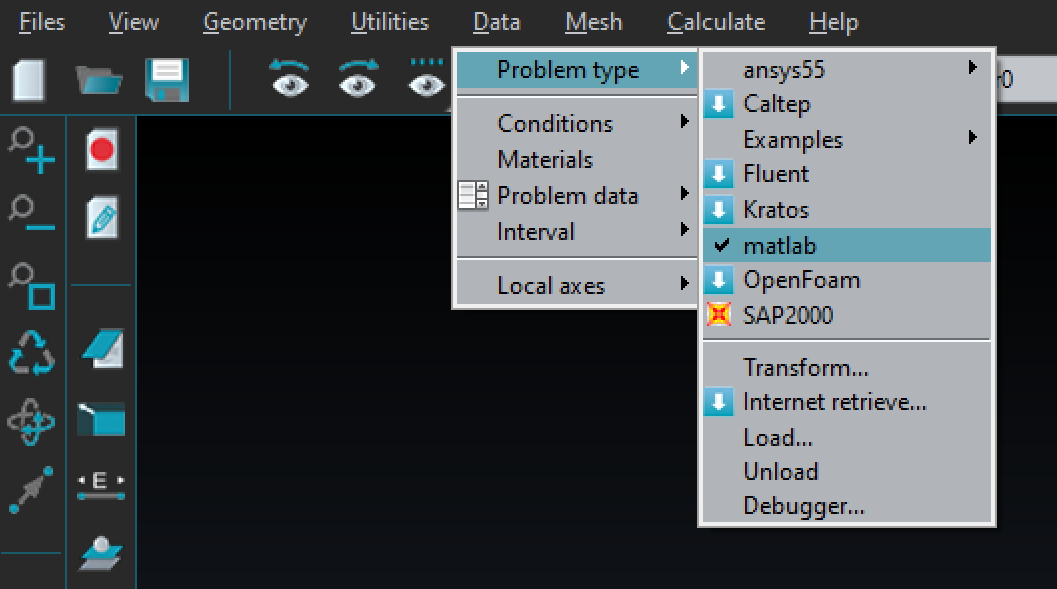
\includegraphics[width=80mm]{images/GiD_probtype.png}
  \caption{\texttt{Matlab} problem type selection}
  \label{fig:Matlabproblemtype}
\end{figure}
Next, create your geometry using the \texttt{geometry} $\rightarrow$ \texttt{create} menu option.

%%%%%%%%%%%%%%%%%%%%%%% GiD - boundary conditions %%%%%%%%%%%%%%%%%%%%%%%%
\subsubsection{Boundary Conditions}
Once the geometry is created, the user must apply boundary conditions in order to constrain the model. Click \texttt{Data} $\rightarrow$ \texttt{Conditions} $\rightarrow$ \texttt{Constraints}, and the menu shown in Figure \ref{fig:GiDConstraints} will appear. For a plane stress problem, only $x$ and $y$ constraints should be applied. In the example discussed in this paper, a value of 0.0 was used for each.\\[3pt]
\begin{figure}[ht]
  \centering
  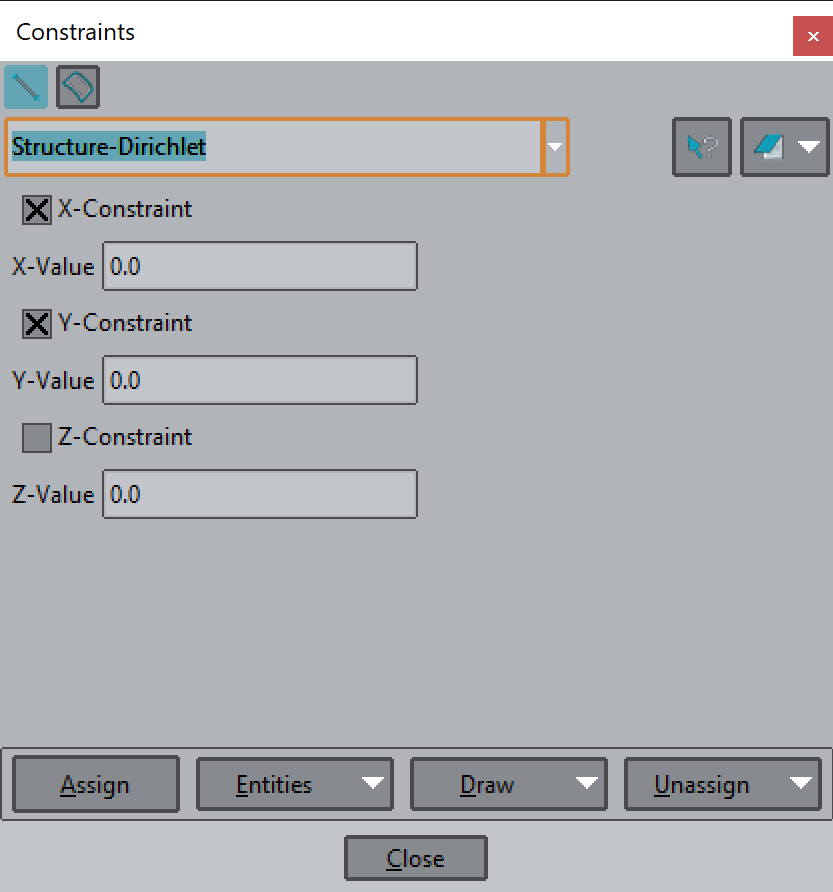
\includegraphics[width=50mm]{images/GiD_constraints.png}
  \caption{constraints menu}
  \label{fig:GiDConstraints}
\end{figure}
Next, click \texttt{Assign} and then click on the edge of the model to apply the desired constraint.

%%%%%%%%%%%%%%%%%%%%%%%%%%%%% GiD - loads %%%%%%%%%%%%%%%%%%%%%%%%%%%%%%%%%
\subsubsection{Loads}
The first modification made to GiD was to allow for the application of point loads. The primary purpose for this was to simplify equation \ref{eqn:responsefctderivative}. The term $\dv{\textbf{P}}{x_i}$ represents the change in the force vector, $\textbf{P}$, with respect to the design variables, $x_i$. This term vanishes if the force vector is constant with respect to the design variables, which is the case when a point load is applied. This simplified equation would make initial implementation and validation of the numerical and analytical sensitivity equations a bit easier.\\[3pt]
The ability to apply a distributed load was already contained within the \texttt{Matlab} problem type. To apply a load after the geometry creation and boundary conditions' assignment, simply click on the \texttt{Data} heading, then \texttt{conditions} $\rightarrow$ \texttt{loads}. The menu shown in Figure \ref{fig:GiDLoadsDist} will appear. There are only two actions that need to be taken. First, select the proper function handle. There is a \texttt{computeConstantVerticalLoad} and a \texttt{computeConstantHorizontalLoad} option. They correspond to functions within the Matlab code hierarchy that assign a constant vertical or horizontal load, respectively. In these functions, the user can input the desired load magnitude. Second, click \texttt{Assign}. Then, select the edge of the structure on which to apply the distributed load.\\[3pt]
\begin{figure}[ht]
  \centering
  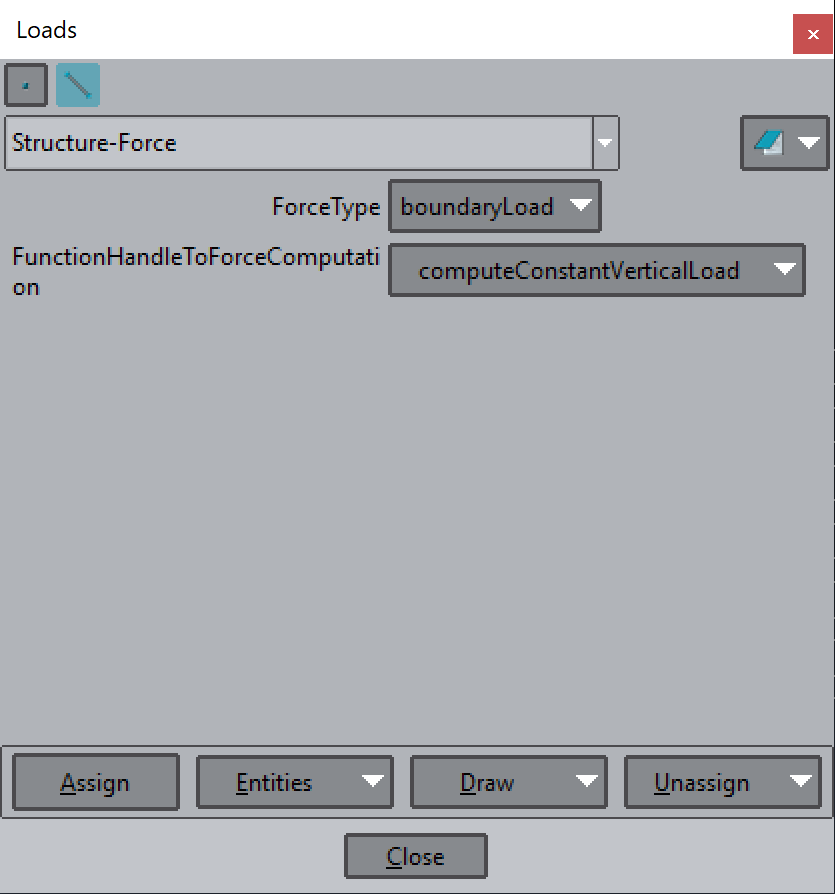
\includegraphics[width=50mm]{images/GiD_loads_dist.png}
  \caption{distributed loads menu}
  \label{fig:GiDLoadsDist}
\end{figure}
In addition to being able to apply a distributed load, the user can apply a point load. This is the functionality added to aid the development of the sensitivity analysis program. The associated menu is also under \texttt{Data} $\rightarrow$ \texttt{Conditions} $\rightarrow$ \texttt{Loads}. Simply click on the symbol in the upper left of the menu to toggle between point and distributed loads. See Figure \ref{fig:GiDLoadsPoint}. Before applying a point load, the mesh must first be generated! The most simple way to generate a mesh in GiD is to click \texttt{Mesh} $\rightarrow$ \texttt{Generate mesh}. Then, enter the desired element size. \textbf{Note:} too small of a mesh size will cause long calculation times.

\begin{figure}[ht]
  \centering
  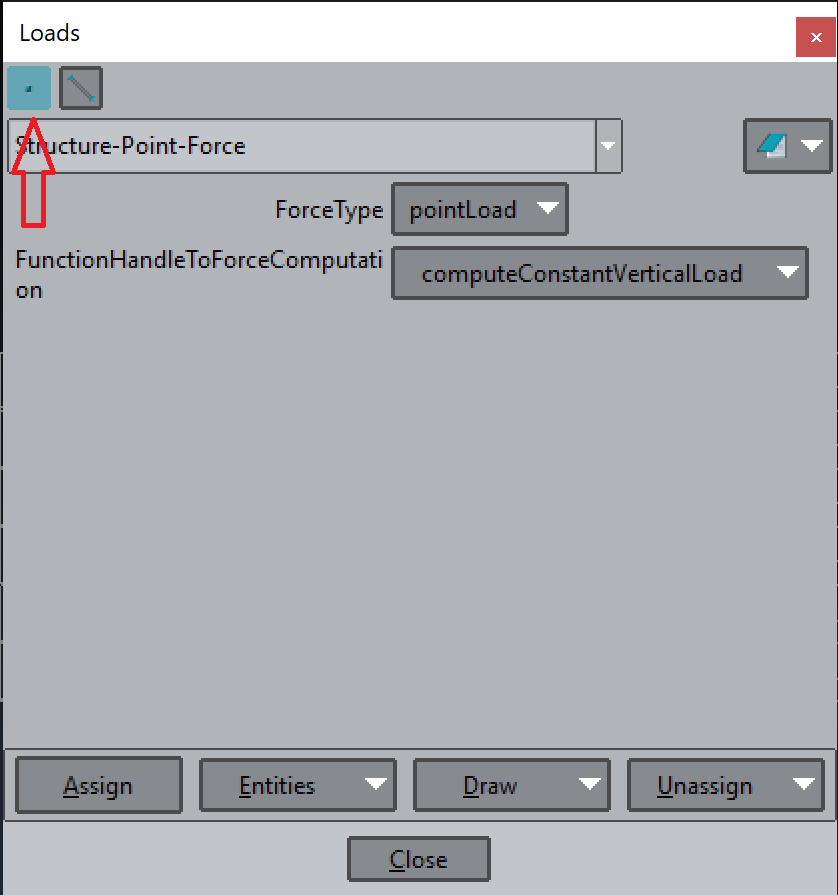
\includegraphics[width=50mm]{images/GiD_loads_point.png}
  \caption{point loads menu}
  \label{fig:GiDLoadsPoint}
\end{figure}
%%%%%%%%%%%%%%%%%%%%%%%% GiD - sensitivity analysis %%%%%%%%%%%%%%%%%%%%%%
\subsubsection{Sensitivity Analysis}
To define the sensitivity analysis parameters, click \texttt{Data} $\rightarrow$ \texttt{Problem Data} $\rightarrow$ \texttt{Sensitivity Analysis}. The menu shown in Figure \ref{fig:GiDSensAnalMenu} will appear. In the upper dropdown menu, the user can select the type of sensitivity analysis. The options are: \texttt{global}, \texttt{numerical adjoint}, and \texttt{analytical adjoint}. Exercise caution when selecting the global method - please ensure a relatively low number of nodes (less than ~200) is used. In the sensitivity analysis menu, the user can click the box next to the desired objective functions. Please note that currently, the von Mises stress objective function only works with the global method due to time constraints. Next, the user can select the finite differencing method: \texttt{forward}, \texttt{backward}, or \texttt{central}. Finally, the user can select the perturbation size. Based on the perturbation study discussed in section \ref{section:perturbationstudy}, a perturbation of $10^{-5}$ worked reliably.
\begin{figure}[ht]
  \centering
  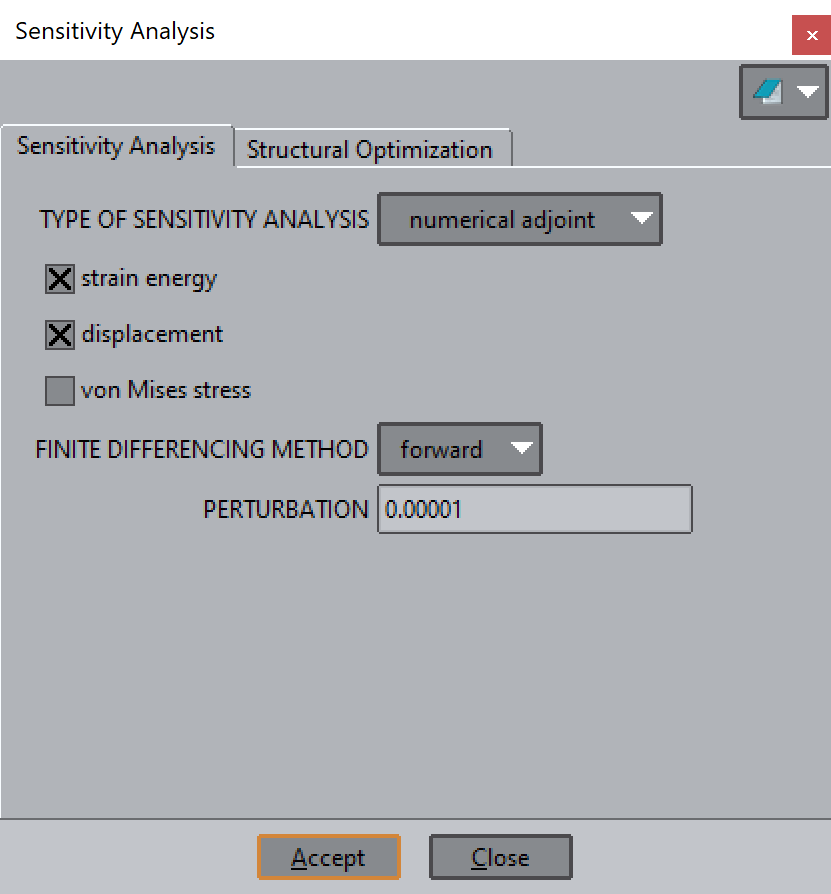
\includegraphics[width=50mm]{images/GiD_sens_analysis.png}
  \caption{sensitivity analysis menu}
  \label{fig:GiDSensAnalMenu}
\end{figure}

%%%%%%%%%%%%%%%%%%%%%%%%%%%% GiD - domains %%%%%%%%%%%%%%%%%%%%%%%%%
\subsubsection{Domains}
Next, click \texttt{Data} $\rightarrow$ \texttt{Conditions} $\rightarrow$ \texttt{Domains}. The menu shown in Figure \ref{fig:GiDDomainsMenu} will appear. In the dropdown menu, click \texttt{Structure-Nodes}, click \texttt{Assign}, select all nodes, and click \texttt{Finish}. Click \texttt{Structure-Elements} in the dropdown menu and perform the same steps.\\[3pt]
Next, parameters associated with the sensitivity analysis must be specified. These are also visible in Figure \ref{fig:GiDDomainsMenu} If a displacement sensitivity analysis is selected, then the user must specify which node(s) on which to perform the analysis. Simply click \texttt{Structure Nodes for Displacement Sensitivity}, \texttt{Assign}, and then select the appropriate node(s). The same steps apply to von Mises stress, except the user must select one or more elements instead of nodes. For a strain energy sensitivity analysis, no further action is needed since the analysis is applicable to the entire structure.
\begin{figure}[ht]
  \centering
  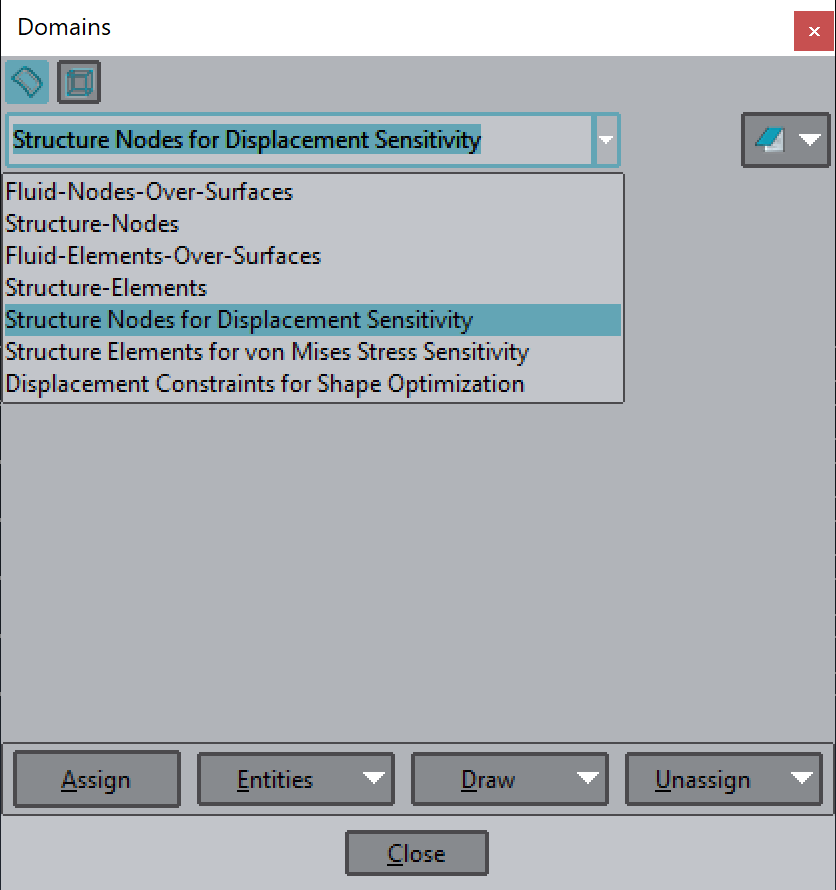
\includegraphics[width=50mm]{images/GiD_domains.png}
  \caption{domains menu}
  \label{fig:GiDDomainsMenu}
\end{figure}
%%%%%%%%%%%%%%%%%%%%%%%%%%%% GiD - materials %%%%%%%%%%%%%%%%%%%%%%%%%
\subsubsection{Material Properties}
Next, the user should input the material properties of the created geometry. Click \texttt{Data} $\rightarrow$ \texttt{Materials}, and the menu shown in Figure \ref{fig:GiDMaterialsMenu} will appear. Make sure to select \texttt{Structure} in the dropdown menu. Enter values appropriate for the type of material being simulated. Next, click \texttt{Assign} and draw a rectangle around all elements. Click \texttt{Finish}.

\begin{figure}[ht]
  \centering
  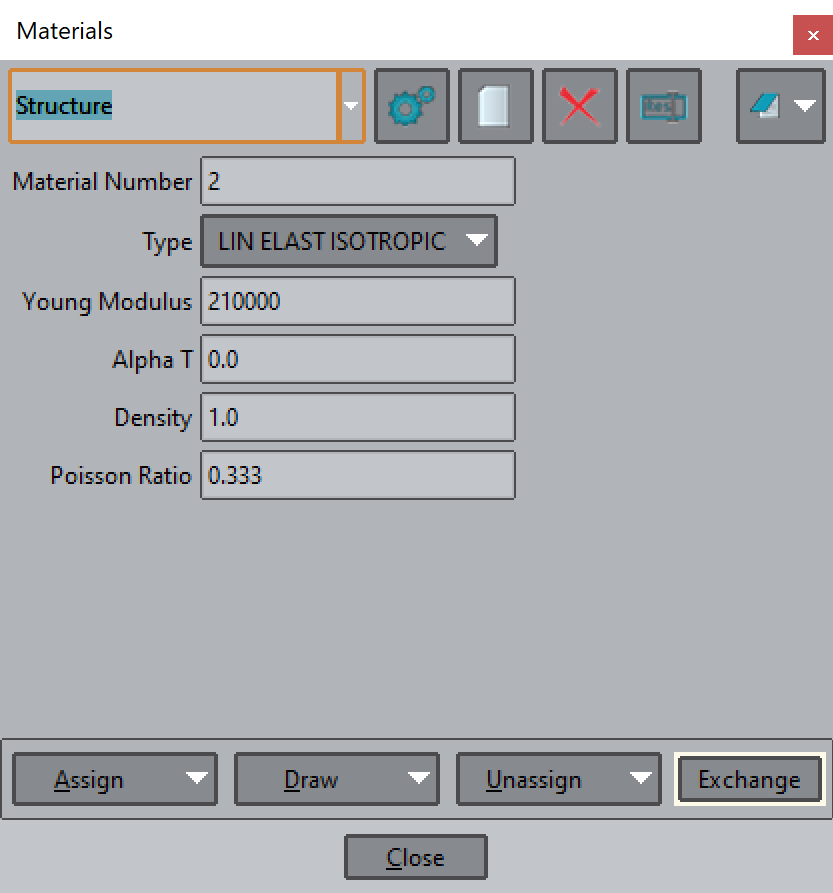
\includegraphics[width=50mm]{images/GiD_materials.png}
  \caption{material properties menu}
  \label{fig:GiDMaterialsMenu}
\end{figure}

%%%%%%%%%%%%%%%%%%%%%%%%%%%% GiD - optimization %%%%%%%%%%%%%%%%%%%%%%%%%
\subsubsection{Optimization}
If the user wants to execute the optimization algorithm, it can be found under \texttt{Data} $\rightarrow$ \texttt{Problem Data} $\rightarrow$ \texttt{Sensitivity Analysis}. Then select the \texttt{Structural Optimization} tab at the top of the menu. See Figure \ref{fig:GiDOptimizationMenu}. The user can specify the sensitivity analysis type, objective function, displacement direction, differencing method, perturbation, number of iterations, and factor of change. For the problem discussed in this paper, the recommended number of iterations is 10, and the recommended factor of change is 5. All other parameters have been discussed previously. Please note that the ideal value of the various inputs will depend on the geometry defined in GiD.\\[3pt]
\begin{figure}[ht]
  \centering
  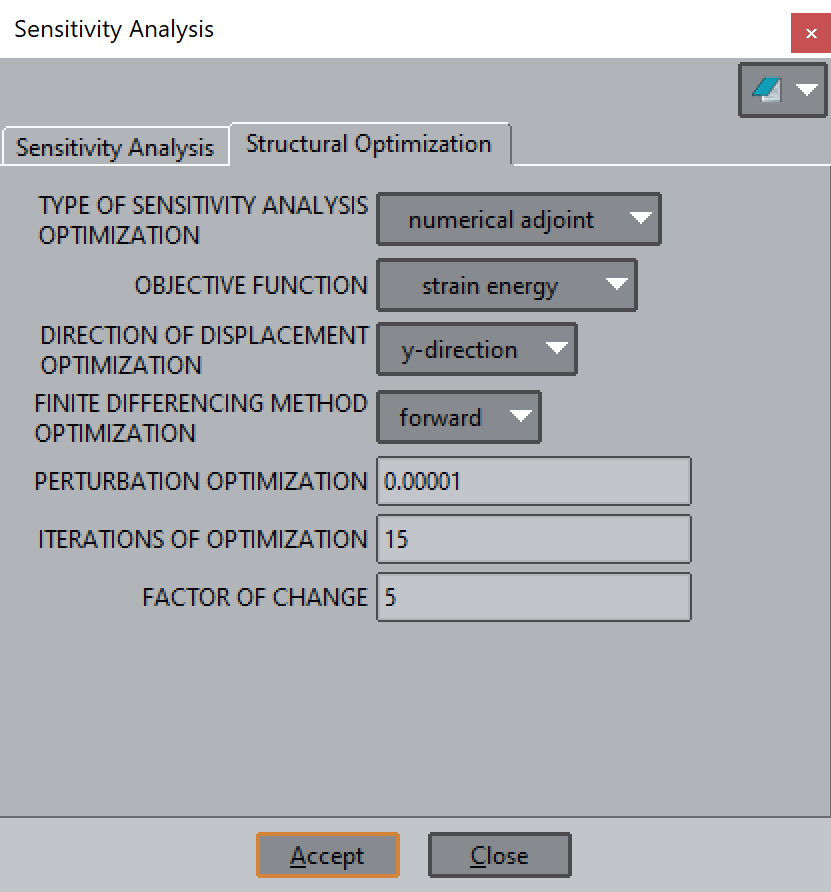
\includegraphics[width=50mm]{images/GiD_optimization.png}
  \caption{optimization menu}
  \label{fig:GiDOptimizationMenu}
\end{figure}
The optimization algorithm could be improved, as mentioned in Section \ref{section:optimization}. It is currently unstable if too many iterations are utilized; therefore, for the problem in this paper, it is best to keep the iteration number at or below 10. The ideal factor of change will likely vary depending on the absolute size of the geometry created in GiD.

%%%%%%%%%%%%%%%%%%%%%%%%%%%% GiD - output %%%%%%%%%%%%%%%%%%%%%%%%%
\subsubsection{Output}
Now that all of the necessary information has been entered into GiD, ensure that the current file has been saved. Then, click \texttt{Calculate} $\rightarrow$ \texttt{Calculate}. This will generate a folder ending in \texttt{.gid}. There will be a \texttt{.dat} file within this folder. This file is what is read in from Matlab in the \texttt{main.m} driver file.  
\subsection{Step-by-step problem solution algorithm} 
\begin{enumerate}
\item Open GiD GUI
\item Click \texttt{Data} $\rightarrow$  \texttt{Problem type} $\rightarrow$ \texttt{matlab}
\item Click \texttt{Geometry} $\rightarrow$  \texttt{create} menu and create your own geometry.
\item Assign boundary conditions under \texttt{Data} $\rightarrow$ \texttt{Conditions} $\rightarrow$ \texttt{Constraints}, click \texttt{Assign} and then click on the model edge to apply.
\item Generate mesh under \texttt{Mesh} $\rightarrow$ \texttt{Generate mesh}, enter the element size and apply.
\item Apply loads, clicking \texttt{Data} $\rightarrow$ \texttt{Conditions} $\rightarrow$ \texttt{Loads} (here you can choose either a point or a distributed load).
\item Define the sensitivity analysis, clicking on \texttt{Data} $\rightarrow$ \texttt{Problem Data} $\rightarrow$ \texttt{Sensitivity Analysis}, then choose your desired analysis method and the objective function, then select your perturbation size and press \texttt{Accept}.  
\item Click \texttt{Data} $\rightarrow$ \texttt{Conditions} $\rightarrow$ \texttt{Domains} $\rightarrow$ \texttt{Structure-Nodes} $\rightarrow$ \texttt{Assign}, then select all nodes and click \texttt{Finish}. Do the same steps with elements of the structure, clicking \texttt{Structure-Elements}. Specify parameters, clicking \texttt{Structure Nodes for Displacement Sensitivity/Structure Elements for von Mises Stress Sensitivity} $\rightarrow$ \texttt{Assign} and select the appropriate nodes/elements.
\item Input the material properties, clicking \texttt{Data} $\rightarrow$ \texttt{Materials}, select \texttt{Structure} in the dropdown menu, enter appropriate values, click \texttt{Assign}, select all elements and click \texttt{Finish}.
\item If optimization is to be done, click \texttt{Data} $\rightarrow$ \texttt{Problem Data} $\rightarrow$ \texttt{Sensitivity Analysis}, select the \texttt{Structural Optimization} tab at the top of the menu, specify the given parameters, click \texttt{Accept}.
\item Save the current file and click \texttt{Calculate} $\rightarrow$ \texttt{Calculate}.
\item Go to the \texttt{main} folder and open the .m file inside in MatLab.
\item  In the section \texttt{Parse data from GiD input file } put the name of your case (the name of the generated .dat file) under \texttt{CaseName=}.
\item Run the problem and obtain the initial configuration figure.
\item Go to ParaView, click \texttt{File} $\rightarrow$ \texttt{Open}, open the \texttt{outputVTK} folder and click on \texttt{FEMPlateInMembraneActionAnalysis} folder afterwards.  
\item Depending on the result of interest you can choose between folders: \texttt{CaseName\textunderscore Optimized\textunderscore Analysis, \newline CaseName\textunderscore Sensitivity\textunderscore Analysis} or \texttt{CaseName\textunderscore Structural\textunderscore Analysis}, where you can see the results of the optimization study, of the sensitivity analysis or the displacements, stresses (including von Mises stress) and strains of the structural analysis correspondingly, changing the parameters in the dropdown menu, as shown on Figure 30.
\end{enumerate}
  \begin{figure}[ht]
  \centering
  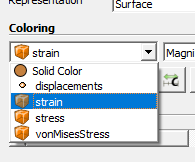
\includegraphics[width=50mm]{images/Paraview.png}
  \caption{ParaView visualization menu}
  \label{fig:Paraview visualization}
\end{figure}
Good luck with the applications; we hope you enjoy it!